% PLEASE DO NOT PLAY WITH ALL THESE SETTINGS, UNLESS YOU REALLY KNOW WHAT YOU ARE DOING. 

%IF YOU HAVE ANY QUESTIONS PLEASE CONTACT: Oscar Vega <ovega@csufresno.edu>

%LaTeX file, comments, and Fresno State formatting created and developed by Brent Alexander Wilson: snahhan@gmail.com.
%Thanks to Dr. Gerardo Munoz for initially creating the formatting of the title, approval, and authorization for reproduction pages.
%Last Updated: November 2012 (GM).
%Last Modified: Oscar Vega, August 2021.
\documentclass[12pt,leqno]{article}\usepackage[pdftex]{graphicx}\usepackage[usenames,dvipsnames]{xcolor}
% maxwidth is the original width if it is less than linewidth
% otherwise use linewidth (to make sure the graphics do not exceed the margin)
\makeatletter
\def\maxwidth{ %
  \ifdim\Gin@nat@width>\linewidth
    \linewidth
  \else
    \Gin@nat@width
  \fi
}
\makeatother

\definecolor{fgcolor}{rgb}{0.345, 0.345, 0.345}
\newcommand{\hlnum}[1]{\textcolor[rgb]{0.686,0.059,0.569}{#1}}%
\newcommand{\hlsng}[1]{\textcolor[rgb]{0.192,0.494,0.8}{#1}}%
\newcommand{\hlcom}[1]{\textcolor[rgb]{0.678,0.584,0.686}{\textit{#1}}}%
\newcommand{\hlopt}[1]{\textcolor[rgb]{0,0,0}{#1}}%
\newcommand{\hldef}[1]{\textcolor[rgb]{0.345,0.345,0.345}{#1}}%
\newcommand{\hlkwa}[1]{\textcolor[rgb]{0.161,0.373,0.58}{\textbf{#1}}}%
\newcommand{\hlkwb}[1]{\textcolor[rgb]{0.69,0.353,0.396}{#1}}%
\newcommand{\hlkwc}[1]{\textcolor[rgb]{0.333,0.667,0.333}{#1}}%
\newcommand{\hlkwd}[1]{\textcolor[rgb]{0.737,0.353,0.396}{\textbf{#1}}}%
\let\hlipl\hlkwb

\usepackage{framed}
\makeatletter
\newenvironment{kframe}{%
 \def\at@end@of@kframe{}%
 \ifinner\ifhmode%
  \def\at@end@of@kframe{\end{minipage}}%
  \begin{minipage}{\columnwidth}%
 \fi\fi%
 \def\FrameCommand##1{\hskip\@totalleftmargin \hskip-\fboxsep
 \colorbox{shadecolor}{##1}\hskip-\fboxsep
     % There is no \\@totalrightmargin, so:
     \hskip-\linewidth \hskip-\@totalleftmargin \hskip\columnwidth}%
 \MakeFramed {\advance\hsize-\width
   \@totalleftmargin\z@ \linewidth\hsize
   \@setminipage}}%
 {\par\unskip\endMakeFramed%
 \at@end@of@kframe}
\makeatother

\definecolor{shadecolor}{rgb}{.97, .97, .97}
\definecolor{messagecolor}{rgb}{0, 0, 0}
\definecolor{warningcolor}{rgb}{1, 0, 1}
\definecolor{errorcolor}{rgb}{1, 0, 0}
\newenvironment{knitrout}{}{} % an empty environment to be redefined in TeX

\usepackage{alltt}
\usepackage{amsmath,amssymb,comment,amsthm}
\usepackage{latexsym}
\usepackage{nextpage}
%\usepackage[pdftex]{graphicx}   %just in case graphicx is not enough... shouldn't need this
\usepackage{graphicx}
\usepackage{thmtools}
\usepackage{float}
\usepackage{array,multirow,hhline}%for tricky things with tables

%%%%%%%%%%%%%%%%%%%%%%%%%%%%%%%%%%%%%%%%%%%%%%%%%%%%%%%%%%%%%%%%%%
%%%%%%%%%%%%%%%%%%%%%%%%%%%%%%%%%%%%%%%%%%%%%%%%%%%%%%%%%%%%%%%%%%
%%%%%%%%%%%                                        Fresno State Formatting Requirements Begins                                  %%%%%%%%%%%%
%%%%%%%%%%%%%%%%%%%y%%%%%%%%%%%%%%%%%%%%%%%%%%%%%%%%%%%%%%%%%%%%%%%
%%%%%%%%%%%%%%%%%%%%%%%%%%%%%%%%%%%%%%%%%%%%%%%%%%%%%%%%%%%%%%%%%%

\usepackage{tocloft} %For table of contents.
\usepackage{verbatim} %Allows us to use \setcounter for manipulating pages
\usepackage{setspace} %Lets user change line spacing of text: normal, 1.5x, and double
\usepackage{indentfirst} %Allow first paragraph to be indented in sections/subsections
\usepackage[font=normal,labelfont=normal,labelsep=period,tableposition=top,justification=raggedright]{caption} %Do a little magic to captions
\usepackage{flafter} %Ensure floats (tables/figures) are never placed before their references.
\usepackage{mathrsfs} %For math symbols -- script L for luminosity
\usepackage{ragged2e} %Used to enable command \raggedright
%\usepackage[compact]{titlesec} %Used for titlespacing command.

\clubpenalty10000
\widowpenalty10000
%those are for avoiding orphan lines at top of pages

\raggedright%Enables left adjust of all text and gets rid of hyphenation throughout the paper, which is required for Fresno formatting.

%This disables bold text on section titles and sets the spacing before & after of section title


\makeatletter
\renewcommand\section{\@startsection {section}{1}{\z@}%
{-3.5ex \@plus -1ex \@minus -.2ex}%
{2.3ex \@plus.2ex}%
{\normalfont\centering}}
\makeatother




%This disables bold text on subsection titles and sets the spacing before & after of section title
\makeatletter
\renewcommand\subsection{\@startsection {subsection}{1}{\z@}%
{-3.5ex \@plus -1ex \@minus -.2ex}%
{0.8pt plus 2pt minus 2pt}%
{\normalfont}}
\makeatother

%This disables bold text on subsubsection titles and sets the spacing before & after of section title
\makeatletter
\renewcommand\subsubsection{\@startsection {subsubsection}{1}{\z@}%
{-3.5ex \@plus -1ex \@minus -.2ex}%
{0.8pt plus 2pt minus 2pt}%
{\normalfont}}
\makeatother

\newcommand{\usubsection}[1]{\subsection[#1]{\centering\normalfont\underline{#1}}}% This underlines sub-sections -- must use \usubsection in paper to identify!
\newcommand{\usubsubsection}[1]{\subsubsection[#1]{\normalfont\normalfont\underline{#1}}}% This underlines sub-sub-sections -- must use \usubsubsection in paper to identify!

\setcounter{tocdepth}{2}%Don't show subsubsections in the Table of Contents:
\setcounter{secnumdepth}{-1}%Disables chapter, section, and subsection numbering
\setlength{\parindent}{0.5in}%Paragraphs must be indented 1/2"
\setlength{\cftbeforefigskip}{0.3cm}% Space between elements of the List of Figures
\setlength{\cftbeforetabskip}{0.3cm}% Space between elements of the List of Tables
\setlength{\cftbeforesecskip}{0.3cm}% Space before Section entries in the Table of Contents
\setlength{\cftbeforesubsecskip}{0.3cm}% Space before Sub-Section entries in the Table of Contents
\setlength\headsep{12pt}%Change spacing between page number and top of text
\setlength{\cftfignumwidth}{1.5em}%Change space between Figure X and the caption for it on the List of Figures
\setlength{\cfttabnumwidth}{1.5em}%Change space between Table X and the caption for it on the List of Tables

\renewcommand{\contentsname}{TABLE OF CONTENTS} %Renames table of contents to how you want it:
\renewcommand{\cfttoctitlefont}{\centering\normalfont}%Change Table of Contents title to be normal & not bold
\renewcommand{\cftsecleader}{\cftdotfill{\cftdotsep}}%This gives you the dots for the table of contents page:
\renewcommand{\listtablename}{LIST OF TABLES}%Renames table of tables to how you want it:
\renewcommand{\cftlottitlefont}{\centering\normalfont}%Change List of Tables title to be normal & not bold
\renewcommand{\cfttabfont}{Table }%Renames "1" on list of tables to "Table 1":
\renewcommand{\listfigurename}{LIST OF FIGURES}%Renames table of figures to how you want it:
\renewcommand{\cftloftitlefont}{\centering\normalfont}%Change List of Figures title to be normal & not bold
\renewcommand{\cftfigfont}{Figure }%Renames "1" on list of figures to "Figure 1":
\renewcommand{\refname}{REFERENCES}%Renames references to how you want it:
\renewcommand{\cftfigaftersnum}{.}%Add a period after Figure X in List of Figures
\renewcommand{\cfttabaftersnum}{.}%Add a period after Table X in List of Tables

%Use this to put page numbers at top right of page
\usepackage{fancyhdr}
\fancyhf{}
\renewcommand{\headrulewidth}{0pt} % remove the header rule
\rhead{\thepage}
\pagestyle{fancy}
\fancyheadoffset[HR]{0.02in}%Moves (horizontally) the page number                              
%KEEP ALL THIS TOGETHER

% Change Table of Content section headers and page numbers to normal instead of bold font
\renewcommand{\cftsecfont}{\normalfont}
\renewcommand{\cftsecpagefont}{\normalfont}

%%Change margins \marginsize{left}{right}{top}{bottom}:
\usepackage{anysize}
\marginsize{1.7in}{1in}{1.2in}{1.6in}

%%%%%%%%%%%%%%%%%%%%%%%%%%%%%%%%%%%%%%%%%%%%%%%%%%%%%%%%%%%%%%%%%%
%%%%%%%%%%%%%%%%%%%%%%%%%%%%%%%%%%%%%%%%%%%%%%%%%%%%%%%%%%%%%%%%%%
%%%%%%%%%%%%                                   Fresno State Formatting Requirements Ends                                   %%%%%%%%%%%%%
%%%%%%%%%%%%%%%%%%%%%%%%%%%%%%%%%%%%%%%%%%%%%%%%%%%%%%%%%%%%%%%%%%
%%%%%%%%%%%%%%%%%%%%%%%%%%%%%%%%%%%%%%%%%%%%%%%%%%%%%%%%%%%%%%%%%%

%%%%%%%%%%%%%%%%%%%%%%%%%%%%%%%%%%%%%%%%%%%%%%%%%%%%%%%%%%%%%%%%
%BEGIN OF MATH SYMBOLS AND COMMANDS
% You, most probably, don't need all what follows. Comment out whatever you don't need to better run LaTeX.
\usepackage[all]{nowidow} %this is to avoid orphan lines
\usepackage{array}
\usepackage[usenames,dvipsnames]{xcolor}
\usepackage{tikz}
%\usepackage{subfigure}

\newtheorem{lemma}{Lemma}%[chapter]
\newtheorem{theorem}[lemma]{Theorem}
\newtheorem{corollary}[lemma]{Corollary}
\newtheorem{proposition}[lemma]{Proposition}
\newtheorem{defnition}[lemma]{Definition} %leave this as is, soon this will be redefined as a new environment
\newtheorem{example}[lemma]{Example}
\newenvironment{definition}{\begin{defnition} \em}{\end{defnition}}

\theoremstyle{remark}
\newtheorem{remark}[theorem]{Remark}

\newcommand{\close}[1]{\begin{equation} #1 \tag*{$\Box$} \end{equation}}

\newcommand{\wtilde}{\widetilde}
\newcommand{\what}{\widehat}
\newcommand{\n}{\noindent}
\renewcommand{\bar}{\overline}
%\newcommand{\qed}{\hfill $\square$}%%%%%%%%%%%%%%%%%%%%%%% use \qed to get square at the end of proofs.
%\newcommand{\proof}{\n \emph{\underline{Proof}} \ : \ }
\newcommand{\rbox}{\hfill $\Box$}
\newcommand{\rdef}{\mbox{} \hfill $\rhd$}
\newcommand{\la}{\langle}
\newcommand{\ra}{\rangle}
\newcommand{\normal}{\unlhd}
\newcommand{\subnormal}{\unlhd \unlhd}
\newcommand{\kar}{\stackrel{\mathrm{char}}{\normal}}
\newcommand{\lra}{\Leftrightarrow}
\newcommand{\labelpar}[1]{\label{#1}}
\newcommand{\Image}{\mbox{\rm Im} \,}
\newcommand{\Ker}{\mbox{\rm Ker} \,}
\renewcommand{\Im}{\mbox{\rm Im} \,}
\newcommand{\deq}{\stackrel{\mathrm{def}}{=}}
\newcommand{\ds}{\displaystyle}
\newcommand{\tst}{\textstyle}
\newcommand{\mbf}{\mathbf}
\newcommand{\mbb}[1]{\mbox{\boldmath$#1$}}
\newcommand{\con}{\, | \,}
\newcommand{\mb}[1]{{\mathbb #1}}
\newcommand{\ip}[2]{\left\langle #1, #2 \right\rangle}
\newcommand{\solution}{\emph{Solution : }}
\newcommand{\answer}[1]{\begin{center} \framebox{#1} \end{center}}
\newcommand{\eps}{\varepsilon}
\newcommand{\boxform}[1]{\medskip \mbox{} \hfill #1 \hfill $\Box$}
\newcommand{\der}[2]{\ds{\frac{\partial #1}{\partial#2}}}
\newcommand{\se}[1]{\setlength{\extrarowheight}{#1}}
\newcommand{\Der}[2]{\frac{\partial #1}{\partial#2}}
\newcommand{\Aut}{\mbox{\rm Aut}}
\newcommand{\Out}{\mbox{\rm Out}}
\newcommand{\Inn}{\mbox{\rm Inn}}
\newcommand{\Sym}{\mbox{\rm Sym}}
\newcommand{\Alt}{\mbox{\rm Alt}}
\newcommand{\GL}{\mbox{\rm GL}}
\newcommand{\PGL}{\mbox{\rm PGL}}
\newcommand{\SL}{\mbox{\rm SL}}
\newcommand{\PSL}{\mbox{\rm PSL}}
\newcommand{\SU}{\mbox{\rm SU}}
\newcommand{\PSU}{\mbox{\rm PSU}}
\newcommand{\symp}{\mbox{\rm Sp}}
\newcommand{\psymp}{\mbox{\rm PSp}}
\newcommand{\unit}{\mbox{\rm U}}
\newcommand{\orth}{\mbox{\rm O}}
\newcommand{\proj}{\mbox{\rm P}}
\newcommand{\Syl}{\mbox{\rm Syl}}
\newcommand{\End}{\mbox{\rm End}}
\newcommand{\rank}{\mbox{\rm rank}}
\newcommand{\Sol}{\mbox{\rm Sol}}
\newcommand{\Fit}{\mbox{\rm Fit}}
\newcommand{\Frat}{\mbox{\rm Frat}}
\newcommand{\Matr}{\mbox{\rm Matr}}
\newcommand{\rad}{\mbox{\rm rad}}
\newcommand{\ord}{\mbox{\rm ord}}
\newcommand{\Fix}{\mbox{\rm Fix}}
\newcommand{\N}{\mathbb{N}}
\newcommand{\F}{\mathbb{F}}
%\newcommand{\emptypage}{\newpage \thispagestyle{empty} \begin{tabbing} just an empty page  \kill \end{tabbing}}
\renewcommand{\liminf}{ \underline{\lim} \,}
\renewcommand{\limsup}{\overline{\lim} \,}
\renewcommand{\iff}{\Leftrightarrow}
\renewcommand{\Re}[1]{\mbox{\rm Re}(#1)}
\renewcommand{\Im}[1]{\mbox{rm Im}(#1)}
\newcommand{\Log}{\mbox{\rm Log} \, }
\newcommand{\hs}{\hspace{1mm}}
\newcommand{\tcr}{\textcolor{red}}
%\renewcommand{\thetable}{\Roman{table}}  To make tables numbered using roman numerals
\newcommand*\mycirc[1]{
\begin{tikzpicture}[baseline=(C.base)]
\node[draw,circle,inner sep=1pt](C) {#1};
\end{tikzpicture}}
%%%%%%%%%%%%%%%%%%%%%%%%%%%%%%%%%%%%%%%%%%%%%%%%%%%%%%%%%%%%%%%%
%END OF MATH SYMBOLS AND COMMANDS

%%%%%%%%%%%%%%%%%%%%%%%%%%%%%%%%%%%%%%%%%%%%%%%%%%%%%%%%%%%%%%%%

\IfFileExists{upquote.sty}{\usepackage{upquote}}{}
\begin{document}
%%%%%%%%%%%%%%%%%%%%%%%%%%%%%%%%%%%%%%%%%%%%%%%%%%%%%%%%%%%%%%%%
\begin{center}
ABSTRACT
\end{center}

\begin{center}
%ABSTRACT TITLE
%SAME TITLE AS TITLE PAGE, SINGLE-SPACED IF OVER \newline
%ONE LINE, TYPED IN INVERTED PYRAMID FORM
Predicting NCAA March Madness Outcomes
\end{center}

\doublespacing
The aim of this project is to develop a machine learning framework to predict outcomes for the NCAA Division I Mens Basketball Tournament. The purpose is to build upon traditional statistical rankings by implementing an automated pipeline that generates precise win probabilities for every possible tournament matchup. Extensive research into historical sports forecasting and modern machine learning techniques was conducted to establish a baseline for predictive accuracy and model calibration.

Following a comprehensive review of existing literature, the models were constructed using R. The primary dataset includes historical game results and Massey Ordinals, supplemented by custom feature engineering designed to capture team momentum and efficiency metrics. Four different modeling techniques were evaluated on the training data: Logistic Regression, Linear Regression, Random Forest, and XGBoost.
 
Unlike standard classification tasks, the final model was evaluated based on its ability to minimize the Brier Score, ensuring that the predicted probabilities were well calibrated against actual tournament results. The findings indicate that the integration of ensemble methods and strength of schedule adjustments provides a competitive edge in forecasting the high variance environment of the tournament. The complete codebase and dataset configurations are hosted on GitHub for further research and reproducibility. (do i put the link here or somewhere else)

%The abstract should fit on one page. A blank guard sheet should follow. Neither of these pages receives a page number, and neither is considered part of the project proper. 

\singlespacing
\vskip 0.3in
\noindent Jonathen Marin%ABSTRACT AUTHOR NAME

\noindent May 2026 %Use May or December, depending on the semester you graduate, even though the deadline is earlier than that.
\thispagestyle{empty}
\newpage

%%%%%%%%%%%%%%%%%%%%%%%%%%%%%%%%%%%%%%%%%%%%%%%%%%%%%%%%%%%%%%%%
%BLANK PAGE AFTER ABSTRACT
\mbox{}
\thispagestyle{empty}
\newpage

%%%%%%%%%%%%%%%%%%%%%%%%%%%%%%%%%%%%%%%%%%%%%%%%%%%%%%%%%%%%%%%%
\begin{center}
%PROJECT TITLE THAT EXTENDS OVER ONE LINE TYPED IN INVERTED PYRAMID FORM. JUST LIKE IN ABSTRACT
Predicting NCAA March Madness Outcomes
\end{center}

\vskip 2in

\begin{center}
by
\end{center}

\begin{center}
Jonathen Marin%AUTHOR'S FULL NAME
\end{center}

\vskip 2in

\begin{center}
A project \\[6pt]
submitted in partial \\[6pt]
fulfillment of the requirements for the degree of \\[6pt]
Master of Science in Mathematics \\[6pt]
in the College of Science and Mathematics \\[6pt]
California State University, Fresno
\end{center}

\begin{center}
May 2026 %CHECK DATE
\end{center}
\setcounter{page}{1}
\pagenumbering{roman}
\thispagestyle{empty}
\newpage

%%%%%%%%%%%%%%%%%%%%%%%%%%%%%%%%%%%%%%%%%%%%%%%%%%%%%%%%%%%%%%%%
\begin{center}
APPROVED
\end{center}

\begin{center}
For the Department of Mathematics:
\end{center}

%Note: Do not use academic titles (i.e., Dr., Ph.D.) when you enter your committee members' names on this page.  Use first and last name only.  When filling in the department name, do not use "Department of"  Simply use Mathematics.  Laser-print this page.  Inkjet print is not acceptable.  Once your committee members have signed, you can bring it to the Graduate Office (Madden Library 4th floor) and I will secure the dean's signature for you.  Delete this box after you have read the instructions.

\noindent
%We use the quote to move the block of text over so it looks nice and aligned with lines below
\begin{quote}
We, the undersigned, certify that the project of the following student meets the required standards of scholarship, format, and style of the university and the student's graduate degree program for the awarding of the master's degree.
\end{quote}

\vskip 0.5in

\begin{center}
Jonathen Marin  %TYPE STUDENT'S NAME THERE. TYPED SAME AS ON TITLE PAGE
\vskip -0.1in
\makebox[\textwidth]{\hspace{4pc}\hrulefill\hspace{4pc}}
Project Author
\end{center}

\vskip 0.5in

\begin{center}
 \makebox[\textwidth]{\hspace{2pc}\hrulefill\hspace{2pc}}
 \end{center}
 \vskip -0.2in
 \hspace{2pc}%TYPE CHAIRPERSON'S  NAME THERE
Earvin Balderama (Chair) \hfill Mathematics  \hspace{2pc}

%THE REST SHOW UP IN ALPHABETICAL ORDER

\vskip 0.3in
\begin{center}
 \makebox[\textwidth]{\hspace{2pc}\hrulefill\hspace{2pc}}
 \end{center}
 \vskip -0.2in
 \hspace{2pc}%TYPE COMMITTEE MEMBER NAME THERE
Patrick Chung \hfill Mathematics  \hspace{2pc}

\vskip 0.3in
\begin{center}
\makebox[\textwidth]{\hspace{2pc}\hrulefill\hspace{2pc}}
\end{center}
\vskip -0.2in
\hspace{2pc}%TYPE COMMITTEE MEMBER NAME THERE
Mario Bañuelos \hfill Mathematics \hspace{2pc}   %TYPE DEPARTMENT NAME OR PROFESSIONAL AFFILIATION, IN CASE COMMITTEE MEMBER IS NOT IN THE DEPARTMENT OF MATHEMATICS

\thispagestyle{empty}
\newpage

%%%%%%%%%%%%%%%%%%%%%%%%%%%%%%%%%%%%%%%%%%%%%%%%%%%%%%%%%%%%%%%%
\begin{center}
ACKNOWLEDGMENTS
\end{center}
\doublespacing

I would like to thank my advisor, Dr. Dvisor, for her helpful advice, guidance, knowledge, and overall general brilliance. It was an honor for me to have the chance to work with such a great mind. I would also like to thank all project committee members for, hopefully, having read my work and asking easy questions at my defense. I  also thank my parents....
\newline\newline\newline

\singlespacing
\thispagestyle{empty}
\newpage

%%%%%%%%%%%%%%%%%%%%%%%%%%%%%%%%%%%%%%%%%%%%%%%%%%%%%%%%%%%%%%%%
\addtocontents{toc}{\hfill Page\par}%This adds text "Page" to Table of Contents

%This creates the table of contents page automatically
\begin{center}
\tableofcontents
\end{center}
\thispagestyle{empty}
\newpage



%TRY TO KEEP YOUR LIST OF TABLES AND FIGURES TO ONE PAGE EACH. IF NOT POSSIBLE, THEN PLEASE CONTACT THE GRADUATE COORDINATOR AS THIS TEMPLATE WILL NEED TO BE MODIFIED TO FIT UNIVERSITY REGULATIONS.

%IF YOU DO NOT HAVE TABLES OR FIGURES, DELETE THE CORRESPONDING PAGE THAT LISTS THEM.

%%%%%%%%%%%%%%%%%%%%%%%%%%%%%%%%%%%%%%%%%%%%%%%%%%%%%%%%%%%%%%%%
\addtocontents{lot}{\hfill Page\par}%This adds text "Page" to List of Tables

%This creates the list of tables page automatically
\addcontentsline{toc}{section}{LIST OF TABLES} %This adds List of Tables to table of contents
\begin{center}
\listoftables
\end{center}
\thispagestyle{empty}
\newpage

%%%%%%%%%%%%%%%%%%%%%%%%%%%%%%%%%%%%%%%%%%%%%%%%%%%%%%%%%%%%%%%%
\addtocontents{lof}{\hfill Page\par}%This adds text "Page" to List of Figures

%This creates the list of figures page automatically
\addcontentsline{toc}{section}{LIST OF FIGURES} %This adds List of Figures to table of contents
\begin{center}
\listoffigures
\end{center}
\thispagestyle{empty}
\newpage



%%%%%%%%%%%%%%%%%%%%%%%%%%%%%%%%%%%%%%%%%%%%%%%%%%%%%%%%%%%%%%%%
\doublespacing%From now on everything will be in double spacing

\begin{center}
\section{INTRODUCTION}
\end{center}
\setcounter{page}{1}%THIS IS TO RESET PAGE NUMBERING SO THAT THE FIRST SECTION IS PAGE 1. NO ROMAN NUMERALS ANYMORE. 
\pagenumbering{arabic}%WE DON'T WANT ROMAN NUMERALS, SO WE SWITCH TO ARABIC.
\thispagestyle{empty} %NO PAGE NUMBER ON SECTION PAGES.
The National Collegiate Athletic Association (NCAA) serves as the premier developmental system for the National Basketball Association (NBA) and the Women's National Basketball Association (WNBA). With thousands of athletes across both divisions arriving from around the world, the influence of the NCAA is extensive. As the basketball world has evolved into a multibillion dollar industry \cite{Berkowitz2025}, the value of a competitive edge has become substantial. Teams historically relied on live scouting and film study to gain these advantages. However, the last decade has seen a major shift toward statistical findings. Inspired largely by the movie \textit{Moneyball}, teams now look to analytics to uncover value that the naked eye might miss. 

The focal point of this competitive landscape is March Madness. At the conclusion of the regular season, the selection committee invites 68 teams to participate in this tournament. The field includes the champions from all 32 Division I conferences alongside the best remaining teams chosen at large. The committee seeds these participants into four distinct regions with rankings ranging from 1 to 16. The four teams judged to be the strongest are awarded the number 1 seeds while the next tier receives the number 2 seeds. Within each region, the teams compete in a single elimination format where matchups are initially determined by rank. For example, the top seed plays the sixteenth seed. The winner of each region advances to the Final Four to compete for the national championship. Crucially, these contests take place at neutral sites rather than on home courts. This structure creates a predictive challenge where volatility is the norm.

To evaluate these predictive challenges in a rigorous and competitive environment, this project utilizes the Kaggle March Machine Learning Mania competition as its primary experimental framework. Kaggle provides a unique platform where data scientists from across the globe compete to minimize error in tournament forecasts using historical data stretching back to 1985. Unlike traditional bracket challenges that reward binary picks, this competition requires the submission of win probabilities for every possible matchup in the tournament field. This shift from simple selection to probabilistic estimation allows for a more granular analysis of model performance and calibration. By using this structured setting, the research can leverage standardized datasets including team efficiency ratings and historical results to build a pipeline that is both reproducible and statistically sound.

This statistical consistency is possible because basketball is uniquely suited for machine learning applications. Both individual and collective performances are captured through a standardized set of metrics. Discrete variables such as points, steals, assists, and rebounds provide a consistent numerical foundation for analysis across different eras and levels of competition. This uniformity allows for the creation of structured datasets where team strength can be quantified and compared through objective performance indicators. By leveraging these recurring statistical patterns, machine learning models can identify underlying trends that govern game outcomes and team efficiency.

A basic assessment often relies on a record of wins and losses to infer the overall quality of a team. While these records serve as strong indicators, they frequently fail to capture critical nuance. Furthermore, the single elimination structure of the tournament ensures that upsets remain a constant possibility regardless of historical dominance. A defining example occurred in \date{2018} when the top ranked Virginia Cavaliers entered the postseason with 31 wins and only 3 losses. They fell to the lowest ranked UMBC Retrievers by 20 points. Such outcomes demonstrate why simple heuristics fail in this environment. 

This inherent volatility drives a massive secondary market focused on sports betting. As legal wagering expands globally, March Madness has evolved into one of the largest gambling events in the world with $3.1$ billion dollars wagered in $2025$ on tournament outcomes \cite{AGA2025}. To manage this risk, bookmakers generate odds which serve as the industry standard for predictive accuracy. These odds represent a market consensus that attempts to price in every available variable from player injuries to historical trends. However, these lines are often influenced by public sentiment and profit margins rather than pure probability. Consequently, developing a model capable of outperforming these market established baselines represents the gold standard for predictive success.

This paper aims to construct a predictive framework capable of meeting this standard. The primary objective is to develop and evaluate distinct statistical models that minimize the Brier Score metric used in the Kaggle competition. By testing various algorithms against historical data, the research seeks to identify a strategy that generates a winning score. The final analysis benchmarks these models against competitor submissions that utilized multiple strategies including elo ratings, standard odds conversion, and analysis rankings. Ultimately, the optimal model will be deployed in the upcoming 2026 March Madness tournament to compare its projections with live results.


Motivated by this challenge, substantial research has addressed the complexities of March Madness prediction. The majority of this work focuses on engineering feature sets for learning algorithms ranging from linear regression to more complex ensemble methods. While the Kaggle competition provides foundational game statistics, transforming these into effective predictors requires significant effort. The following subsection details the specific data types provided by the competition to establish this baseline. The final subsection we review existing literature with a primary focus on feature engineering. Finally, the paper details the implementation of distinct modeling techniques. This comparative analysis examines linear and logistic regression alongside additional statistical methods. These models are compared against one another and evaluated relative to the winning scores from prior competitions.
% NOTE THAT THE TEMPLATE DOES NOT HAVE CHAPTERS, BUT SECTIONS, AND THAT THESE ARE NOT NUMBERED...
\usubsection{Data Available}
The highly quantifiable nature of basketball ensures that statistical data is both abundant and accessible. While the Kaggle competition permits participants to incorporate any external datasets they acquire, the organizers themselves provide a comprehensive archive. This repository includes over 30 distinct tables of historical data spanning more than three decades. All of the tables are separated by gender, with the only exception being the public rankings table. This is due to the fact that they only compiled mens rankings. 

The data provided by Kaggle is split into regular season and postseason files. For the purposes of this project, the tournament phase is referred to as the playoffs. This research focuses primarily on the detailed results tables for both the regular season and the playoffs while also utilizing the essential rankings and seeding tables. Although the broader archive extends further back, the detailed game statistics required for this analysis commence in the 2003 season. Each entry in these tables provides a comprehensive statistical breakdown for both the winning and losing teams in every recorded matchup.

\begin{figure}[H]
\begin{center}
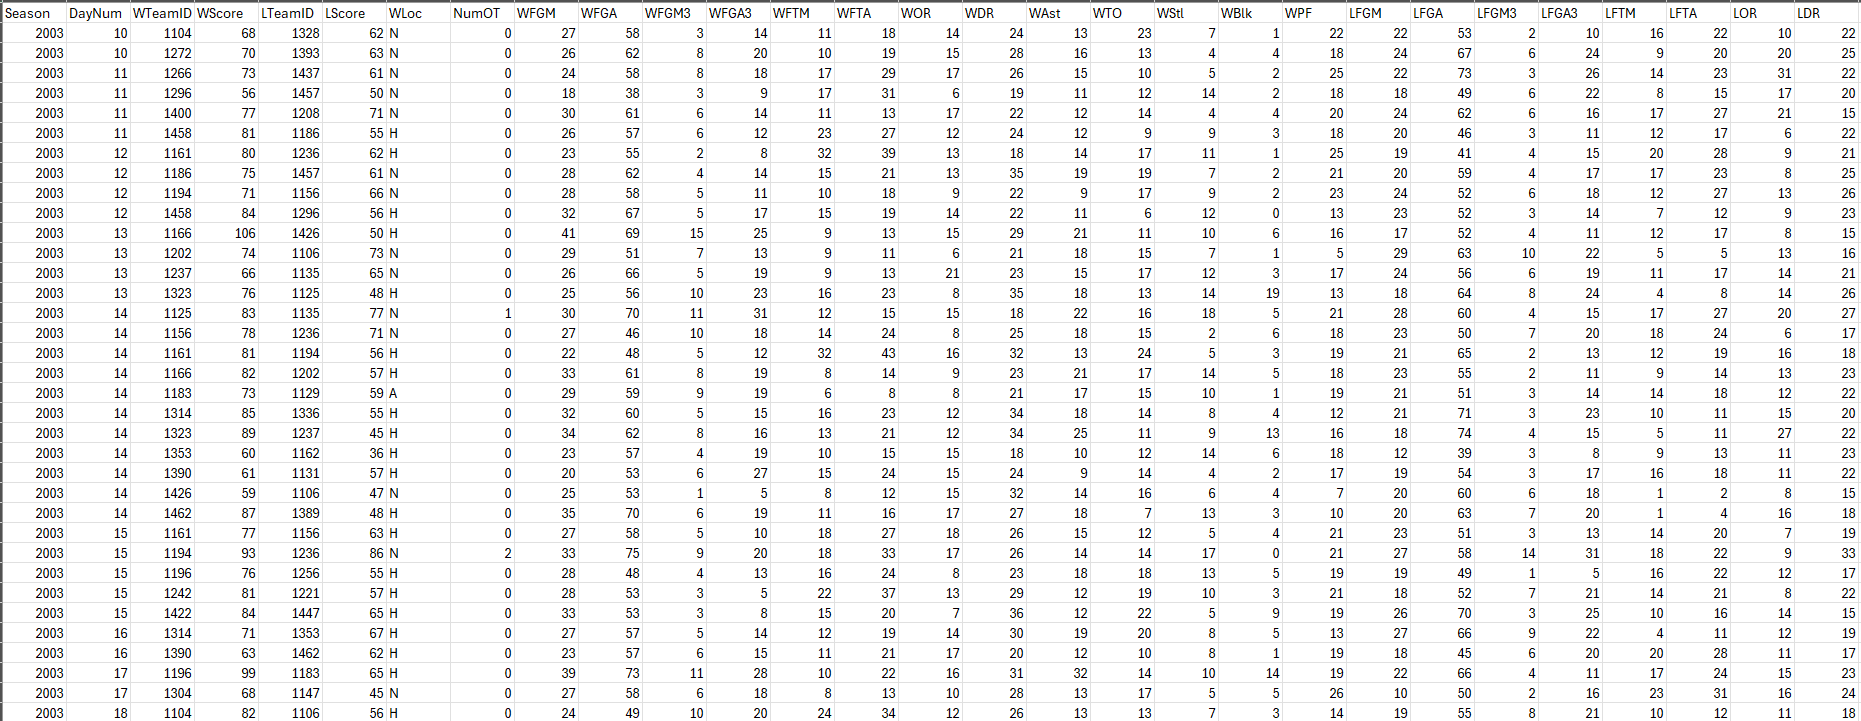
\includegraphics[scale=.3]{paper_photos/regseason.png}
\caption{Regular Season Detailed Data}
\label{regseason}
\end{center}
\end{figure}

This table records key performance metrics for each game played. The schema utilizes the prefix W to denote statistics for the winning team and the prefix L for the losing team. The specific recorded variables include:

\begin{itemize}
    \item Points Scored
    \item The number of field goals made and attempted (FGM-A).
    \item The number of 3-point field goals made and attempted (FGM-A3).
    \item The number of free throws made and attempted (FTM-A).
    \item The number of offensive and defensive rebounds secured (OR- DR).
    \item The number of assists (Ast).
    \item The number of turnovers (TO).
    \item The number of blocks (Blk).
    \item The number of fouls (PF).
\end{itemize}

While raw box scores provide the foundation of events that happened in a game, they often fail to capture nuances in, and out, of the game. To address this limitation, this research supplements the Kaggle datasets with advanced metrics from analyst Ken Pomeroy (KenPom). Pomeroy is accepted as the industry standard for college basketball analysis. Pomeroy's approach is to normalize the data by calculating efficiency rather then raw stats. Theses statistics are updated daily throughout the regular season and tournament. For the purpose of this study, a snapshot of the rankings was acquired from the day prior to the start of the 2025 tournament.  

\begin{figure}[H]
\begin{center}
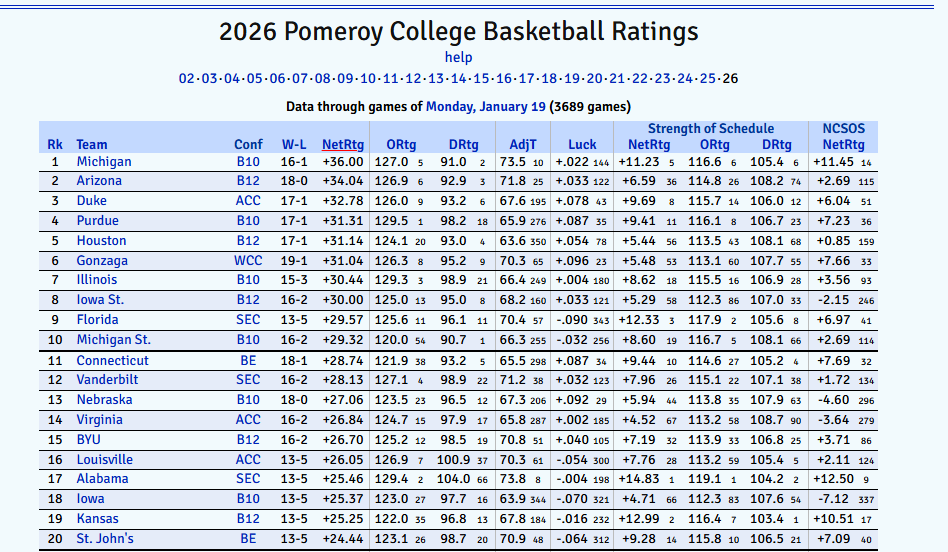
\includegraphics[scale=.5]{paper_photos/kenpom.png}
\caption{The first 20 teams of the KenPom data table.}
\label{kenpom}
\end{center}
\end{figure}

The primary metrics utilized from this source include:
\begin{itemize}
    \item Net Rating (NetRtg).
    \item Offensive Rating (ORtg).
    \item Defensive Rating (DRtg).
    \item Adjusted Tempo (AdjT).
\end{itemize}
Net rating is the differential between Offensive and Defensive Rating. Offensive Rating measures the points scored per $100$ possessions. Similarly, defensive rating measure the points given up per $100$ possessions. These ratings are adjusted by the quality of opponents a team has played, and the game location. Lastly, Adjusted tempo is the number of possessions per $40$ minutes. We define a possession as the period where a team controls the ball, ending with a shot attempt, turnover, or score. 

While Pomeroy's ratings serve as the industry standard, they are exclusively available for the Men's division. Consequently, this research incorporates an additional dataset from Bart Torvik that focuses on the Women's division. Torvik cites Pomeroy as a significant influence; thus, the ratings are constructed using a comparable methodology. However, distinct algorithmic differences exist between the two systems. For further detail regarding these distinctions, the reader is referred to \cite{Torvik}. The metrics used from Barttovik are:
\begin{itemize}
    \item Adjusted Offensive Efficiency (ADJOE).
    \item Adjusted Defensive Efficiency (ADJDE). 
    \item Adjusted Tempo (ADJ T.). 
\end{itemize}

\begin{figure}[H]
\begin{center}
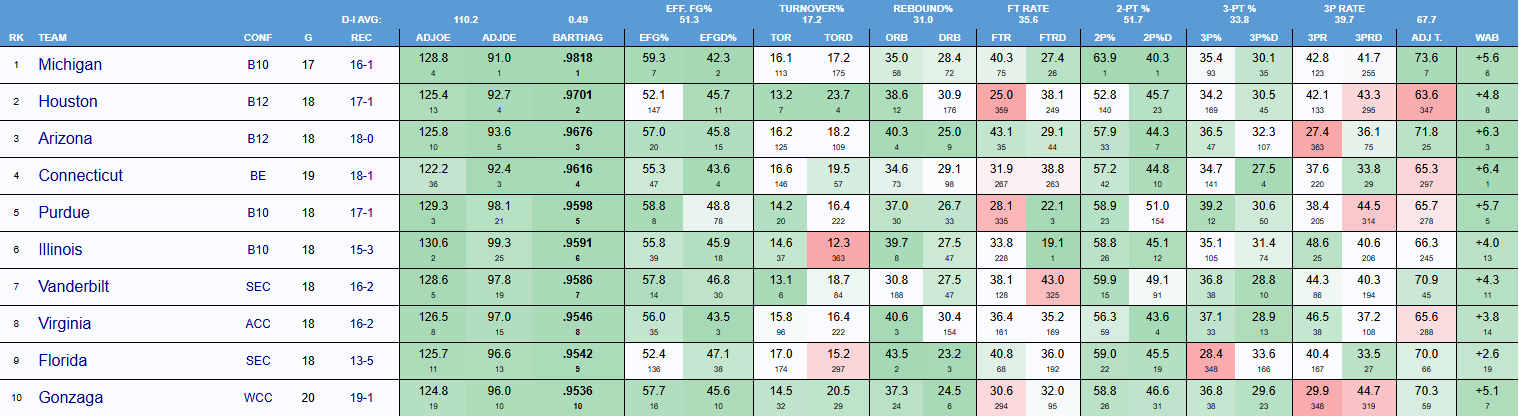
\includegraphics[scale=.35]{paper_photos/bartervik.png}
\caption{The first 10 teams of the Barttorvik table}
\label{barttorvik}
\end{center}
\end{figure}

To complement the efficiency metrics provided by Pomeroy and Torvik, this research also incorporates the comprehensive ranking systems aggregated by Kenneth Massey. While the previously discussed datasets focus on raw predictive efficiency, the Massey Ordinals provide a consolidated view of team hierarchy. This dataset aggregates rankings from over $40$ distinct mathematical systems, pollsters, and algorithms. These rankings typically present data as an ordinal integer where the top team is assigned the value of $1$. Incorporating this data allows the model to leverage a "wisdom of the crowd" approach by utilizing the consensus of the broader analytical community. 

\begin{figure}[H]
\begin{center}
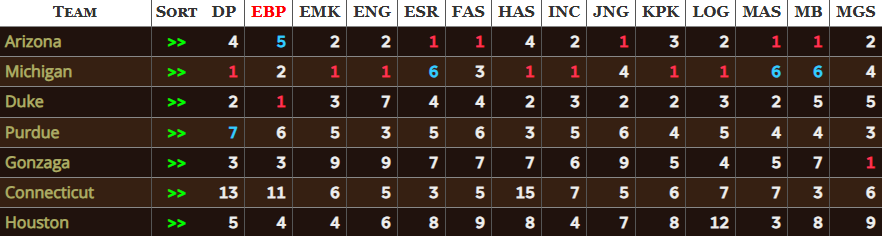
\includegraphics[scale=.5]{paper_photos/massey.png}
\caption{A sample of the Massey Ordinals table showing distinct ranking systems.}
\label{massey}
\end{center}
\end{figure}
One significant challenge in aggregating these distinct sources is the inconsistency in team nomenclature. For instance, a university might be listed as "St. Mary's" in one dataset and "Saint Mary's CA" in another. To resolve this discrepancy, all external data was strictly mapped to the unique TeamID integer provided by the Kaggle competition files. This standardization ensures that the advanced efficiency metrics are accurately merged with the box score data for every specific matchup.



\newpage
%YOU SHOULD USE STANDARD LaTeX TO TYPESET YOUR WORK. USE \ref AND \cite, DO NOT HARDCODE YOUR REFERENCES.


%%%%%%%%%%%%%%%%%%%%%%%%%%






%THIS IS HOW YOU PLACE FIGURES. PLEASE FOLLOW THIS TEMPLATE SO YOUR PICTURES DO NOT FLOAT TO WHERE YOU DO NOT WANT THEM.

%\begin{figure}[H]
%\begin{center}
%\includegraphics[scale=.7]{rw2dn4.pdf}
%\caption{Probability Distribution Frequencies for $n = 4$}
%\label{2dfrequencies}
%\end{center}
%\end{figure}

%%%%%%%%%%%%%%%%%%%%%%%%%%%
%\usubsection{A Third Subsection with an Equation}





%NOTE THAT ABOVE, I FINISHED THE PROOF WITH  \qedhere. THIS IS SO THE SQUARE IS ON THE SAME LINE AS THE LAST LINE WRITTEN. IF YOU COMMENT THAT OUT, YOU WILL SEE THAT THE SQUARE GOES ONE LINE LOWER, UGLY AND BAD PRACTICE.


%%%%%%%%%%%%%%%%%%%%%%%%%%%%%%%%%%%%%%%%%%%%%%%%%%%%%%%%%%%%%%%%
\begin{center}
\section{LITERATURE REVIEW}
\end{center}
\thispagestyle{empty} %NO PAGE NUMBER ON SECTION PAGES.


\usubsection{Past Strategies}
The pursuit of a perfect bracket has generated a substantial body of research in predictive modeling over the last decade. While specific algorithms vary, the most successful strategies in the Kaggle Machine Learning Mania competition consistently rely on one of two distinct methodological frameworks.

The primary objective for this study is to minimize the Brier Score. We define the Brier Score (BS) as follows:

\begin{equation}
    BS = \frac{1}{N} \sum_{t=1}^N (f_t - o_t)^2
\end{equation}

where $N$ is the number of events, $f_t$ is the predicted probability, and $o_t$ is the actual outcome. For this research, a $0$ is considered a loss, and a $1$ is a win. A Brier Score of $0$ would reflect perfect accuracy, while a Brier Score of $1$ reflects perfect inaccuracy. To provide a baseline, a strategy where we predict every team has a $50\%$ chance of winning would result in a Brier Score of $0.25$. (thinking of putting another example here)

The first framework relies on fundamental analysis where the objective is to construct a ground-truth probability independent of public sentiment. A common implementation of this approach involves utilizing domain-specific heuristics such as the elo rating system. Originally designed for chess, elo provides a dynamic measure of team strength that updates after every game. It offers a robust baseline that accounts for strength of schedule more effectively than raw win-loss records \cite{chess}. Many strategies also incorporate expert features. These include the Nate Silver, FiveThirtyEight, and KenPom ratings which act as high-signal inputs that aggregate player health, travel distance, and roster depth into a single numeric value. By treating these expert outputs as features rather than final predictions, modelers can leverage human domain expertise while correcting for known expert biases.

The second dominant framework relies on the Efficient Market Hypothesis \cite{EMH}. This approach posits that global betting markets, specifically closing lines from major bookmakers, offer a more accurate aggregate predictor of game outcomes than individual statistical models. The efficacy of this strategy is well-documented in recent Kaggle competitions where five of the top eight performing models utilized market-derived features as their primary feature. These strategies do not attempt to beat the market. Instead, they focus on mathematically disentangling the true win probability from the bookmaker's overround and inherent biases.

To achieve this, recent state-of-the-art implementations utilize specific conversion algorithms to de-noise betting data. The standard tool in this domain is the $\textit{Goto\_conversion}$. Competitors employ these functions to address the favorite-longshot bias. This is the tendency for markets to overvalue underdogs and undervalue favorites. By applying these corrections, modelers can transform raw Vegas odds into highly calibrated probabilities that minimize Brier Score more effectively than fundamental analysis alone. This approach effectively leverages the crowd wisdom of the market while stripping away the pricing inefficiencies introduced by public betting behavior. For more information on how this strategy works, we refer the reader to \cite{goto}.

The applicability of these methodological frameworks, however, is heavily constrained by the structural discontinuity introduced by the 2021 Name, Image, and Likeness (NIL) legislation. Statistical analysis of the post-NIL landscape reveals a significant deviation from historical norms, characterized by a rapid consolidation of talent where the number of programs with elite win percentages (
$>75\%$) has nearly tripled \cite{CBS}. This phenomenon implies that feature weights derived from pre-2021 eras are likely subject to significant concept drift. Consequently,
this literature review restricts its focus to winning strategies from recent Kaggle competitions (2022-present), as methodologies developed before the NIL era may not reflect the approaches best suited to the heightened stratification of team strength driven by current transfer portal dynamics.
 
\newpage
\usubsection{Modeling Techniques}
Recent tournament prediction methodologies employ several established modeling and computational techniques. This section provides formal definitions for the five core approaches used in this study: Logistic Regression, Linear Regression, Monte Carlo Simulation, Random Forest, and Neural Networks.

Logistic Regression is a binary classification model that estimates the probability of an outcome by applying the logistic (also known as sigmoid) function to a linear combination of input features. The model is defined as:

\begin{equation}
P(Y=1|X) = \frac{1}{1 + e^{-(\beta_0 + \beta_1 x_1 + \beta_2 x_2 + ... + \beta_n x_n)}}
\end{equation}
where $Y$ is the binary outcome, $X = (x_1,x_2,\ldots,x_n)$ represents the feature vector, and $\beta = (\beta_0,\beta_1\, \ldots, \beta_n)$ are the model coefficients estimated through the maximum likelihood estimation. This function ensures the predicted probabilities are bounded between $[0,1]$. Logistic regression assumes a linear relationship between the input features and the log-odds of the outcome. This assumption can be restrictive when the true relationships are nonlinear. To address this limitation, common approaches are feature engineering with polynomial or interaction terms (e.g, $x^2, x_i \cdot x_j)$ to capture nonlinear patterns. 

Linear Regression is a supervised learning method that models the relationship between a dependent variable and one or more independent variables by fitting a linear equation to the observed data. Linear Regression is defined as:
\begin{equation}
\hat{Y} = \beta_0 + \beta_1 x_1 + \beta_2 x_2 + \ldots + \beta_n x_n
\end{equation}
where $\hat{Y}$ is the predicted continuous outcome, $X = (x_1, x_2, \ldots, x_n)$ represents the vector of features, and $\beta = (\beta_0, \beta_1, \ldots, \beta_n)$ are the model coefficients estimated through ordinary least squares (OLS) minimization. For more information on OLS we refer the reader to \cite{OLS}. Unlike logistic regression, linear regression produces unbounded predictions and does not inherently output probabilities. In sports prediction contexts, linear regression is commonly used to estimate point totals, scoring margins, or other continuous performance metrics that can subsequently be transformed into win probabilities through additional techniques.

\begin{figure}[H]
    \centering
    % First Figure
    \begin{minipage}{0.45\textwidth}
        \centering
        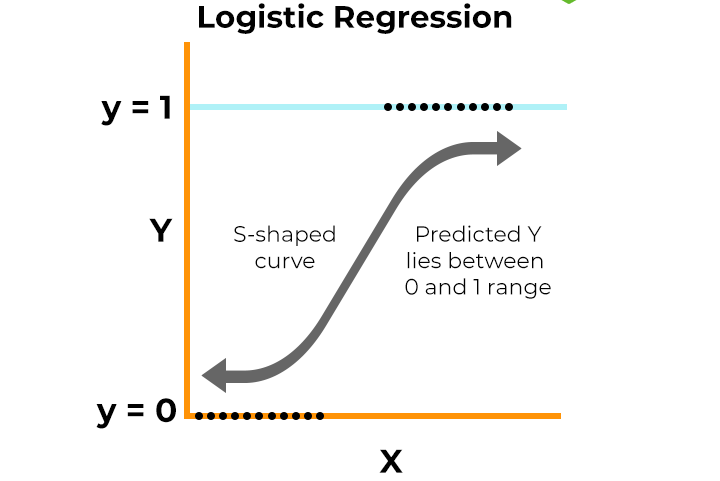
\includegraphics[width=\linewidth]{paper_photos/logisticreg.png}
        \caption{An Example of a Logistic Regression Equation \cite{logphoto}.}
        \label{logistic}
    \end{minipage}\hfill
    % Second Figure
    \begin{minipage}{0.45\textwidth}
        \centering
        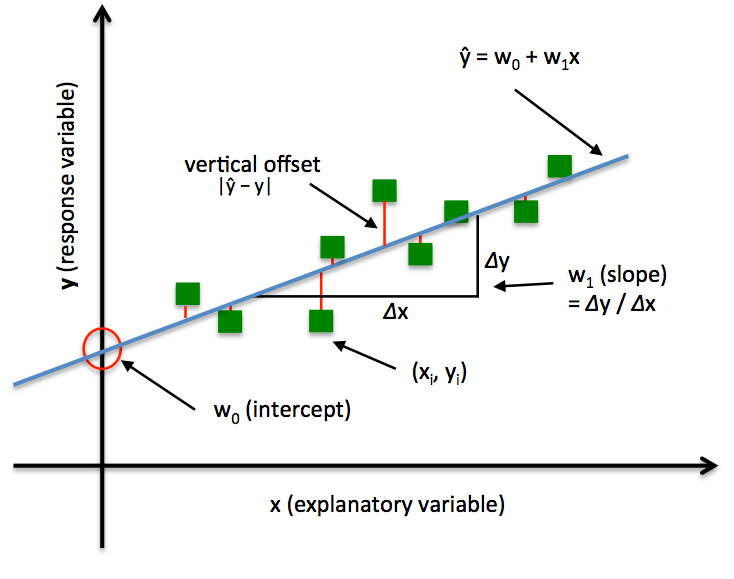
\includegraphics[width=\linewidth]{paper_photos/simple_regression.png}
        \caption{An Example of a Linear Regression Equation \cite{linearphoto}.}
        \label{linear}
    \end{minipage}
\end{figure}

Monte Carlo Simulation is a computational technique that uses repeated random sampling to estimate probabilities for systems with inherent uncertainty. The method generates $N$ independent samples $x_1, x_2, \ldots, x_N$ from a probability distribution $f(x)$, then estimates probabilities by computation the proportion of samples satisfying a certain condition. The simulation is defined as:
\begin{equation}
\hat{P} = \frac{1}{N}\sum_{i=1}^{N} {1}(x_i \in A)
\end{equation}
where $1(\cdot)$ is the indicator function that equals $1$ when the condition is satisfied and $0$ otherwise. $A$ represents the event of interest, and $\hat{P}$ is the Monte Carlo estimate of the true probability $P(A)$. By the Law of Large Numbers \cite{Large Numbers}, $\hat{P} \to P(A)$ as $N \to \infty$. In sports prediction contexts, Monte Carlo methods are frequently employed to simulate game outcomes by sampling from estimated score distributions, enabling the estimation of win probabilities through empirical frequency counts across simulated matchups.

XGBoost (Extreme Gradient Boosting), considered a "black-box" approach, is an ensemble learning method that constructs a sequence of decision trees where each successive tree is trained to correct the residual errors of the previous trees. Unlike Random Forest, which builds trees independently, XGBoost employs gradient boosting to iteratively minimize a loss function through additive modeling \cite{XGBoost}. The model prediction is defined as the sum of predictions from all trees:
\begin{equation}
\hat{y}_i = \sum_{k=1}^K f_k(x_i).
\end{equation} 
Here, $f_k(x_i)$ is the prediction of the $k^{\text{th}}$ tree for the $i^{\text{ith}}$ data point, $\hat{y}_i$ is the final predicted value for the  $i^{\text{ith}}$ data point, and $K$ is the number of trees. Each tree is trained to minimize the objective function 

\begin{equation}
    \text{obj}(\theta) = \sum_{i}^n l(y_i, \hat{y}_i) + \sum_{k=1}^K \Omega(f_k)
\end{equation}
where $l$ is the loss function which simply computes the difference between the true and predicted, and $\Omega$ is the regularization term, discouraging overly complex trees. The optimization process then proceeds via gradient descent on the residuals. For more information regarding gradient descent we refer the reader to \cite{GD}. XGBoost is widely adopted in competitive machine learning for its performance on structured data and ability to capture complex interactions and relationships between features. 

Neural Networks are a class of machine learning models inspired by biological neural systems, consisting of interconnected layers of computational nodes (neurons) that learn hierarchical feature representations through iterative optimization. A feedforward neural network transforms input features through multiple layers of weighted connections and nonlinear activation functions.

For a network with $L$ layers, the output at layer $\ell$ is computed as

\begin{equation}
h^{(\ell)} = \sigma\left(W^{(\ell)} h^{(\ell-1)} + b^{(\ell)}\right)
\end{equation}
if i do neural nets i will keep going with this. 
\newpage

%%%%%%%%%%%%%%%%%%%%%%%%%%%%%%%%%%%%%%%%%%%%%%%%%%%%%%%%%%%%%%%%
\begin{center}
\section{Binary Prediction Models}
\end{center}
\thispagestyle{empty} %NO PAGE NUMBER ON SECTION PAGES.

\usubsection{Data Cleaning}
1 if team A won 0 if team A loss for each game
considering training/testing strategies why i chose what i did (amount of data/ why reg season?) why only that year? 

\usubsection{Variable Selection}
%%%%%%%%%%%%%%%%%%%%%%
\usubsection{Logistic Regression}
\usubsection{Boosting}

\usubsection{Results}


Here are my insights...

\newpage

%%%%%%%%%%%%%%%%%%%%%%%%%%%%%%%%%%%%%%%%%%%%%%%%%%%%%%%%%%%%%%%%
%%%%%%%%%%%%%%%%%%%%%%%%%%%%%%%%%%%%%%%%%%%%%%%%%%%%%%%%%%%%%%%%
\begin{center}
\section{Point Spread Models}
\end{center}
\thispagestyle{empty} %NO PAGE NUMBER ON SECTION PAGES.
same as above
%%%%%%%%%%%%%%%%%%%%%%
\usubsection{s}
Here are my insights...

\newpage

%%%%%%%%%%%%%%%%%%%%%%%%%%%%%%%%%%%%%%%%%%%%%%%%%%%%%%%%%%%%%%%%
%%%%%%%%%%%%%%%%%%%%%%%%%%%%%%%%%%%%%%%%%%%%%%%%%%%%%%%%%%%%%%%%
\begin{center}
\section{Comparison of models}
\end{center}
\thispagestyle{empty} %NO PAGE NUMBER ON SECTION PAGES.

%%%%%%%%%%%%%%%%%%%%%%
\usubsection{My Contributions and Analysis}
Here are my insights...

\newpage

%%%%%%%%%%%%%%%%%%%%%%%%%%%%%%%%%%%%%%%%%%%%%%%%%%%%%%%%%%%%%%%%
%%%%%%%%%%%%%%%%%%%%%%%%%%%%%%%%%%%%%%%%%%%%%%%%%%%%%%%%%%%%%%%%
\begin{center}
\section{2026 Competition}
\end{center}
\thispagestyle{empty} %NO PAGE NUMBER ON SECTION PAGES.

%%%%%%%%%%%%%%%%%%%%%%
\usubsection{Strategies}
Here are my insights...
\usubsection{Results}

\newpage

%%%%%%%%%%%%%%%%%%%%%%%%%%%%%%%%%%%%%%%%%%%%%%%%%%%%%%%%%%%%%%%%

\begin{center}
\section{CONCLUSIONS}
\end{center}
\thispagestyle{empty} %NO PAGE NUMBER ON SECTION PAGES.

%%%%%%%%%%%%%%%%%%%%%%
\usubsection{Summary}

As a preliminary assessment...

\clearpage

%%%%%%%%%%%%%%%%%%%%%%%%%%%%%%%%%%%%%%%%%%%%%%%%%%%%%%%%%%%%%%%%


\begin{thebibliography}{99}
\addcontentsline{toc}{section}{REFERENCES} %THIS ADDS REFERENCES TO TABLE OF CONTENTS
\singlespacing %THIS LOOKS BETTER ON REFERENCE PAGE, DOUBLESPACING WOULD BE TOO UGLY
\thispagestyle{empty} %NO PAGE NUMBER ON SECTION PAGES.

\bibitem{Berkowitz2025} S. Berkowitz. NCAA revenue shattered record in 2024, but association faces massive debt from legal settlements. \emph{USA Today}. (2025). Available at https://www.usatoday.com/story/sports/college/2025/02/27/ncaa-financial-report-revenue-surplus/80733616007/

\bibitem{AGA2025} Cohen, Dara. “Americans to Legally Wager Estimated \$3.1 Billion on March Madness - American Gaming Association.” American Gaming Association, 13 Mar. 2025, www.americangaming.org/americans-to-legally-wager-estimated-3-1-billion-on-march-madness/.

\bibitem{Torvik} Torvik, Bart. “T-Rank FAQ.” Blogspot.com, 2017, adamcwisports.blogspot.com/p/every-possession-counts.html.

\bibitem{GD} IBM. “Gradient Descent.” Ibm.com, 7 Oct. 2021, www.ibm.com/think/topics/gradient-descent.

\bibitem{XGBoost} Kavlakoglu, Eda, and Erika Russi. “XGBoost.” Ibm.com, 9 May 2024, www.ibm.com/think/topics/xgboost.

\bibitem{CBS} Boone, Kyle. “How NIL Has Changed College Basketball: Numbers Deep Dive Reveals Surprising Trends, Recipe for Success.” CBSSports.com, 2025, www.cbssports.com/college-basketball/news/how-nil-has-changed-college-basketball-numbers-deep-dive-reveals-surprising-trends-recipe-for-success/.

\bibitem{Optimization} Melis Kizildemir, et al. “A Family of Solutions Related to Shin’s Model for Probability Forecasts.” Journal of Quantitative Analysis in Sports, vol. 21, no. 2, 6 Feb. 2025, pp. 153–158, https://doi.org/10.1515/jqas-2024-0064. Accessed 20 Jan. 2026.

\bibitem{EMH} Burns, William. “Efficient-Market Hypothesis (EMH) | EBSCO.” EBSCO Information Services, Inc. | Www.ebsco.com, 2024, www.ebsco.com/research-starters/social-sciences-and-humanities/efficient-market-hypothesis-emh.

\bibitem{goto} gotoConversion. “GitHub - GotoConversion/Goto\_conversion: Goto\_conversion - Powered $47,000$ of Prize Money, over $10$ Gold Medals and $100$ Medals on Kaggle.” GitHub, 2025, github.com/gotoConversion/goto\_conversion/tree/main. Accessed 20 Jan. 2026.

\bibitem{chess} Glickman, Mark  E., and Thomas Doan. The US Chess Rating System. 26 July 2025, www.glicko.net/ratings/rating.system.pdf.

\bibitem{OLS} Lumivero. “Ordinary Least Squares Regression (OLS).” XLSTAT, Your Data Analysis Solution, 2025, www.xlstat.com/solutions/features/ordinary-least-squares-regression-ols.

\bibitem{logphoto} Kanade, Vijay. “Everything You Need to Know about Logistic Regression.” Spiceworks Inc, Spiceworks, 8 Apr. 2022, www.spiceworks.com/soft-tech/what-is-logistic-regression/.

\bibitem{linearphoto} Raschka, Sebastian. “LinearRegression: An Implementation of Ordinary Least-Squares Linear Regression - Mlxtend.” Rasbt.github.io, rasbt.github.io/mlxtend/user\_guide/regressor/LinearRegression/.

\bibitem{Large Numbers} “Law of Large Numbers | EBSCO.” EBSCO Information Services, Inc. | Www.ebsco.com, 2022, www.ebsco.com/research-starters/mathematics/law-large-numbers.
%IF YOU ARE DOING A PROJECT IN PURE/APPLIED MATH, THEN YOU NEED TO USE AMS STYLE FOR REFERENCES (GET YOUR REFERENCES FROM MATHSCINET). CONSULT YOUR ADVISOR ABOUT WHAT IS THE STANDARD IN YOUR FIELD, IF YOU ARE DOING STATS OR MATH ED.
\end{thebibliography}
\end{document} 
